\section{Dinamica interna}
Arrivati a questo punto è interessante studiare la dinamica interna di queste galassie, ossia come si muovono le stelle al loro interno. Si nota infatti che le galassie a spirale e quelle ellittiche hanno una dinamica interna molto differente:

\begin{itemize}
    \item \emph{Galassie a spirale:} sono "rotation supported", ossia le stelle si muovono su orbite circolari (o quasi) attorno al centro (in modo molto ordinato). Le misure di cinematica interna si esplicano nella realizzazione di una curva di rotazione, che descrive come la rotazione delle stelle varia con al distanza dal centro galattico.
    \item \emph{Galassie ellittiche:} sono “pressure supported”, ossia le stelle su muovono di moti randomici attorno al centro (moto non ordinato). Una misura di cinematica si traduce nella realizzazione di un profilo di dispersione di velocità. Infatti noi dobbiamo pensare che il sistema si muove con un moto di insieme (il cosidetto "bulk motion") verso di me o lontano da me, ma ciascuna stella ha proprio moto. La dispersione di velocità misura quanto la velocità delle singole stelle sono disperse attorno alla velocità media del bulk motion, anche detta velocità sistemica.
\end{itemize} 

\subsection{Curve di rotazione delle galassie a spirale}
Per analizzare la dinamica interna delle galassie a spirale ci serviamo di due strumenti principali:
\begin{itemize}
    \item Split spettroscopy: mettiamo una fenditura quando osserviamo una galassia, in modo da ricevere solo la luce caduta sulla fenditura: al centro della fenditura ci sarà la luce che proviene dal centro della galassia e la luce ai bordi della fenditura verrà invece dal bordo della galassia. Per costruire uno spettro a questo punto misuriamo una determinata riga spettrale, prima al centro e poi agli estremi della fenditura: quello che si ottiene è che la riga è centrata a lunghezze d’onda diverse per effetto Doppler. La riga della parte di galassia che si avvicina a noi è blue shifted e quella della parte di galassia che si allontana da noi è red shifter e attraverso una misura della differenza delle lunghezze d’onda delle parti estremali trovo la velocità di rotazione della galassia. La riga misurata al centro mi dice invece la velocità sistemica della galassia (tramite un confronto della lunghezza d’onda con quella di laboratorio), come viene riassunto in figura METTI REFERENZA. La velocità di rotazione si misura utilizzando forti righe di emissione in banda otica e dalla riga 21cm in banda radio (viene da idrogeno neutro--gas freddo). 

    \item Integral Field spettroscopy: combina imaging (fotometria) e spettroscopia. Dopo aver ottenuto un’immagine della galassia, da ogni pixel del CCD otteniamo uno spettro. Abbiamo quindi un piano su cui si ha la luce che viene raccolta e una terza dimensione perché per ogni pixel c'è uno spettro. QUesto ci permette di avere informazione sulla dinamica non solo sulla fenditura, come prima, ma su tutta l’area della galassia, quindi riusciamo ad ottenere delle mappe bidimensionali di rotazione. Mentre con la "split spettroscopy" abbiamo un valore di velocità per ogni distanza fissata dal centro, in questo modo otteniamo invece una mappa bidimensionale, quindi in ogni punto dell’area possiamo vedere quanto velocemente ruotano le stelle.
\end{itemize}

\begin{figure}
    \centering
    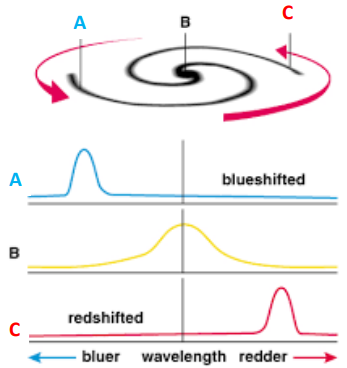
\includegraphics[width = 0.4 \textwidth]{immagini/effetto-doppler.png}
    \caption{La riga proveniente dal punto B (centro della galassia) ci dà la velocità sistemica, mentre le linee che provengono dai punti A e C ci dicono come si stanno muovendo i bracci della galassia: se si muovono verso di noi avranno emissione più spostata sul blu, mentre se si allontanano sul rosso.}
    \label{fig:effetto-doppler-galassie}
\end{figure}

Le stelle in una galassia a spirale sono punti che ruotano attorno al centro, quindi  ci aspettiamo un potenziale kepleriano; la galassia però non è puntiforme. Dobbiamo quindi pensarla come a una sfera di gas e una stella che si muove in quella sfera. Al centro della galassia si ha rotazione nulla (infatti ci troviamo sull'asse di rotazione), poi ci sarà un andamento lineare della velocità fino a un certo punto, in cui possiamo ritornare al caso kepleriano, con un andamento riassunto in figura \begin{comment}\ref{fig:potenziale-galassie-a-spirale}\end{comment}. 

\begin{comment}
\begin{figure}
    \centering
    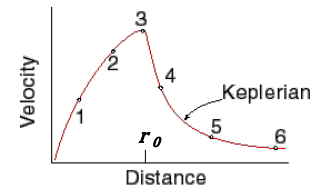
\includegraphics[width = 0.5 \textwidth]{immagini/potenziale-galassie-a-spirale.png}
    \caption{Andamento del potenziale nelle galassie a spirale.}
    \label{fig:potenziale-galassie-a-spirale}
\end{figure}
\end{comment}

%Dal punto 3 di figura \begin{comment}\ref{fig:potenziale-galassie-a-spirale}\end{comment}, siamo fuori dalla zona in cui c’è tanta materia, la densità è così bassa che posso approssimare la situazione come se fosse una massa puntiforme e quindi poi ci aspettiamo un andamento kepleriano Dal profilo di brillanza ci aspetteremo quindi un andamento dapprima con aumento lineare della velocità (fino a quando mi trovo abbastanza vicino alla galassia e più forza d'interazione c'è) e poi decrescita kepleriana.. Guardando ai dati però non si osserva il “calo” kepleriano che ci aspetteremmo da come osserviamo la materia visibile. C'è una spiegazione a questo: l'unico modo per avere un andamento di questo tipo è infatti avere la presenza di una massa invisibile che continua ad essere presente anche quando ci aspettiamo che sia finiti la materia della galassia. Questa materia, che contribuisce alla buca di potenziale ma non è rilevabile attraverso emissione elettromagnetica, viene detta \emph{materia oscura}.